\chapter{Topology}

The concept of topological space grew out of the study of the 
real line and euclidean space and the study of continuous 
functions on these spaces. The information in this chapter is 
based on the second edition of Munkres' \emph{Topology} (2000).

\newpage

%%%%%%%%%%%%%%%%%%%%%%%%%%%%%%%%%%%%%%%%%%%%%%%%%%%%%%%%%%%%%%%%%%

\section{Topological Space}\label{top space}

\begin{definition}[Topology/Open Set/Topological Space]
	A \df{topology}\index{topology} on a set $X$ is a collection 
	$\ms{T}$ of subsets of $X$ called \df{open 
	sets}\index{topology!open 
	set} having the following properties:
	\begin{enumerate}
		\item $\varnothing$ and $X$ are in $\ms{T}$.
		
		\item The union of the elements of any subcollection of 
		$\ms{T}$ is in $\ms{T}$.
		
		\item The intersection of the elements of any finite 
		subcollection of $\ms{T}$ is in $\ms{T}$.
	\end{enumerate}
	
	A \df{topological space}\index{topology!topological space} is 
	an 
	ordered pair $(X,\ms{T})$ consisting of a set $X$ and a 
	topology $\ms{T}$ on $X$. We shorten the statement ``$U$ is 
	an open set containing $x$'' to the phrase ``$U$ is a 
	\df{neighborhood}\index{topology!neighborhood} of $x$.''
\end{definition}

\begin{marginfigure}
	\begin{subfigure}{2in}
		\centering
		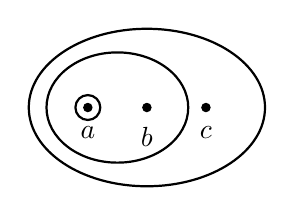
\begin{tikzpicture}
		\draw[thick] (0,0) ellipse (1.5 and 1);
		\filldraw (-.75,0) circle (1.5pt) node[label=below:$a$] 
		(a) {};
		\filldraw (0,0) circle (1.5pt) node[label=below:$b$] (b) 
		{};
		\filldraw (.75,0) circle (1.5pt) node[label=below:$c$] 
		(c) {};
		
		\draw[thick] (a) circle (4.5pt);
		\draw[thick] (-.375,0) ellipse (.9 and .7);
		\end{tikzpicture}
		\caption{These subsets are a topology for $X = \{ a, b, c 
		\}$.}\label{top example}
	\end{subfigure}
	\begin{subfigure}{2in}
		\centering
		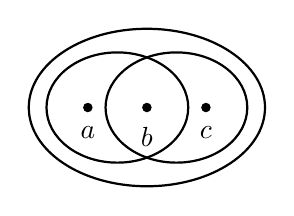
\begin{tikzpicture}
		\draw[thick] (0,0) ellipse (1.5 and 1);
		\filldraw (-.75,0) circle (1.5pt) node[label=below:$a$] 
		(a) {};
		\filldraw (0,0) circle (1.5pt) node[label=below:$b$] (b) 
		{};
		\filldraw (.75,0) circle (1.5pt) node[label=below:$c$] 
		(c) {};
		
		\draw[thick] (-.375,0) ellipse (.9 and .7);
		\draw[thick] (.375,0) ellipse (.9 and .7);
		\end{tikzpicture}
		\caption{These subsets are not a topology for $X = \{ a, 
		b, c \}$.}\label{top nonexample}
	\end{subfigure}
\end{marginfigure}

This is an extremely abstract definition, but the notion of open 
sets will lead to a definition of continuity: a 
generalization of the epsilon-delta definition from analysis. 
(See Section \ref{cont f sect}.) A given set will have more than 
one topology it 
can be equipped with.

\begin{example}
	If $X$ is any set, the collection of all subsets of $X$ is a 
	topology on $X$; it is called the \df{discrete 
	topology}\index{topology!discrete topology}. The collection 
	consisting of $X$ and $\varnothing$ only is also a topology 
	on $X$; it is called the \df{indiscrete 
	topology}\index{topology!indiscrete topology}, or the 
	\df{trivial topology}\index{topology!trivial topology}.
\end{example}

\begin{theorem}
	Let $X$ be a topological space. Then the following conditions 
	hold:
	\begin{enumerate}
		\item[(1)] $\varnothing$ and $X$ are closed.
		
		\item[(2)] Arbitrary intersections of closed sets are 
		closed.
		
		\item[(3)] Finite unions of closed sets are closed.
	\end{enumerate}
\end{theorem}

A bijective correspondence which preserves the topological 
structure is called a homeomorphism. See section 
\ref{homeomorphism}.

%%%%%%%%%%%%%%%%%%%%%%%%%%%%%%%%%%%%%%%%%%%%%%%%%%%%%%%%%%%%%%%%%%

\subsection{Comparing Topologies}

\begin{itemize}
	\item If $\ms{T} \subseteq \ms{T}'$, we say that $\ms{T}'$ is 
	\df{finer}\index{topology!finer} than $\ms{T}$. If $\ms{T} 
	\subsetneq \ms{T}'$, we say that $\ms{T}'$ is \df{strictly 
	finer} than $\ms{T}$. We also say that $\ms{T}$ is (strictly) 
	\df{coarser}\index{topology!coarser} than $\ms{T}'$. $\ms{T}$ 
	and $\ms{T}'$ are \df{comparable}\index{topology!comparable} 
	if $\ms{T} \subseteq \ms{T}'$ or $\ms{T}' \subseteq \ms{T}$.
	
	\item The statement ``$\ms{T}'$ is finer than $\ms{T}$'' is 
	equivalent to the statement ``For each $x \in X$ and each 
	basis element $B \in \ms{B}$ containing $x$, there is a basis 
	element $B' \in \ms{B}'$ such that $x \in B' \subseteq B$.''
\end{itemize}

%%%%%%%%%%%%%%%%%%%%%%%%%%%%%%%%%%%%%%%%%%%%%%%%%%%%%%%%%%%%%%%%%%

\subsection{Generating a Topology}

\begin{definition}[Basis For a Topology]\label{basis top}
	If $X$ is a set, a \df{basis}\index{topology!basis for a} for 
	a topology on $X$ is a collection $\ms{B}$ of subsets of $X$ 
	(called \df{basis elements}) such that
	\begin{enumerate}
		\item[(1)] For each $x \in X$, there is at least one 
		basis element $B$ containing $x$.
		
		\item[(2)] If $x$ belongs to the intersection of two 
		basis elements $B_1$ and $B_2$, then there is a basis 
		element $B_3$ containing $x$ such that $B_3 \subseteq B_1 
		\cap B_2$.
	\end{enumerate}
	If $\ms{B}$ satisfies these two conditions, we define the 
	\df{topology $\ms{T}$ generated by $\ms{B}$} as follows: A 
	subset $U$ of $X$ is open in $X$ if for each $x \in U$, there 
	is a basis element $B \in \ms{B}$ such that $x \in B$ and $B 
	\subseteq U$. Note that each basis element is itself an 
	element of $\ms{T}$.
\end{definition}

\begin{example}If $\ms{B}$ is the collection of all open 
intervals in the real line, the topology generated by $\ms{B}$ is 
called the \df{standard topology}\index{topology!standard 
topology of the real line} of the real line.
\end{example}

\begin{marginfigure}
	\centering
	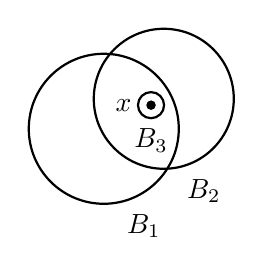
\begin{tikzpicture}
	\node[draw,thick,circle,minimum 
	size=.75in,label={[xshift=.2in]below:$B_1$}] at (0,0) {};
	
	\node[draw,thick,circle,minimum 
	size=.7in,label={[xshift=.2in]below:$B_2$}] at 
	(.3in,.15in) {};
	
	\filldraw (.6,.3) circle (1.5pt) node[label=left:$x$] 
	(x) {};
	\node[draw,circle,thick,label=below:$B_3$] at (.6,.3) 
	{};
	\end{tikzpicture}
	\caption{Illustration of condition (2) of Definition 
		\ref{basis top}}\label{cond 2 fig}
\end{marginfigure}

\begin{itemize}
	\item Let $X$ be a set; let $\ms{B}$ be a basis for a 
	topology $\ms{T}$ on $X$. Then $\ms{T}$ equals the collection 
	of all unions of elements of $\ms{B}$. That is, every open 
	set $U$ in $X$ can be expressed as a union of basis elements.
	
	\item We can obtain a basis for a given topology as follows: 
	Gather a collection $\ms{C}$ of open sets $U$ of $X$ such 
	that for each $x \in U$, there is an element $C$ of $\ms{C}$ 
	such that $x \in C \subseteq U$. $\ms{C}$ is a basis for the 
	topology of $X$.
\end{itemize}

	A \df{subbasis}\index{topology!subbasis} $\ms{S}$ is a 
	collection of subsets of $X$ whose union equals $X$. The 
	\df{topology generated by the subbasis} $\ms{S}$ is defined 
	to be the collection $\ms{T}$ of all unions of finite 
	intersections of elements of $\ms{S}$.
	

%%%%%%%%%%%%%%%%%%%%%%%%%%%%%%%%%%%%%%%%%%%%%%%%%%%%%%%%%%%%%%%%%%
%%%%%%%%%%%%%%%%%%%%%%%%%%%%%%%%%%%%%%%%%%%%%%%%%%%%%%%%%%%%%%%%%%

\newpage

\section{Closed Sets}

\begin{definition}[Closed Set]
	A subset $A$ of a topological space $X$ is said to be 
	\df{closed}\index{topology!closed set} if the set $X 
	\setminus A$ is open.
\end{definition}

A set can be both open and closed, one and not the 
other, or neither.
There are analogous theorems/definitions for closed sets as for 
open sets, and these have been placed alongside the 
theorems/definitions for open sets.

\begin{definition}[Interior and Closure of Set]
	Given a subset $A$ of a topological space, the 
	\df{interior}\index{topology!interior} of $A$ is defined as 
	the union of all open sets contained in $A$, and the 
	\df{closure}\index{topology!closure} of $A$ is defined as the 
	intersection of all closed sets containing $A$. The interior 
	of $A$ is denoted $\Int{A}$, and the closure of $A$ is 
	denoted by $\Cl{A}$ or $\bar{A}$.
\end{definition}

The main idea is that the closure of an open interval is a closed 
interval and the interior of a closed interval is an open 
interval.

\begin{itemize}
	\item We have $\Int{A} \subseteq A \subseteq \bar{A}$.
	
	\item If $A$ is open, $A = \Int{A}$; while if $A$ is closed, 
	$A = \bar{A}$.
\end{itemize}

\begin{theorem}
	Let $A$ be a subset of the topological space $X$.
	\begin{enumerate}
		\item[(a)] Then $x \in \bar{A}$ if and only if every 
		neighborhood of $x$ intersects $A$.
		
		\item[(b)] Supposing the topology of $X$ is given by a 
		basis, then $x \in \bar{A}$ if and only if every basis 
		element $B$ containing $x$ intersects $A$.
	\end{enumerate}
\end{theorem}

\begin{marginfigure}
	\centering
	\begin{tikzpicture}[scale=1.5]
		\draw (0,0) -- (3,0);
		
		\draw[{Bracket[width=2.5mm]}-{Bracket[width=2.5mm]}] 
		(1,0) -- 
		(2.5,0);
		\filldraw (1,0) circle (1pt) node[label=above:$x$] (x) 
		{};
		\draw[decoration={brace},decorate] 
		(1,.1) -- node[above=5pt] {$A$} (2.5,.1);
		
		\draw[{Parenthesis-Parenthesis}] (.75,0) -- (1.25,0);
		\draw[decoration={brace,mirror,raise=5pt},decorate] 
		(.75,0) -- node[below=6pt] {$U_x$} (1.25,0);
	\end{tikzpicture}\caption{Any neighborhood of $x$ intersects 
	$A$, so $x \in \bar{A}$.}\label{th 321 a}
\end{marginfigure}

Part (a) is illustrated in Figure \ref{th 321 a}.

\begin{definition}[Limit Point]
	If $A$ is a subset of the topological space $X$ and if $x$ is 
	a point of $X$, we say that $x$ is a \df{limit 
	point}\index{topology!limit point} of $A$ if every 
	neighborhood of $x$ intersects $A$ in some point other than 
	$x$ itself. Equivalently, $x$ is a limit point of $A$ if it 
	belongs to the closure of $A \setminus \{ x \}$.
\end{definition}

The point $x$ may lie in $A$ or not.

\begin{theorem}
	Let $A$ be a subset of the topological space $X$; let $A'$ be 
	the set of all limit points of $A$. Then
	\[
		\bar{A} = A \cup A'\,.
	\]
\end{theorem}
	
\begin{corollary}
	A subset of a topological space is closed if and only if 
	it contains all its limit points.
\end{corollary}

\begin{theorem}
	Let $X$ be a space satisfying the $T_1$ axiom; let $A$ be a 
	subset of $X$. Then the point $x$ is a limit point of $A$ if 
	and only if every neighborhood of $x$ contains infinitely 
	many points of $A$.
\end{theorem}

\begin{theorem}
	Let $\{ X_\alpha \}$ be an indexed family of spaces; let 
	$A_\alpha \subseteq X_\alpha$ for each $\alpha$. If $\prod 
	X_\alpha$ is given either the product or the box topology, then
	\[
		\prod \bar{A}_\alpha = \overline{\prod A_\alpha}\,.
	\]
\end{theorem}

%%%%%%%%%%%%%%%%%%%%%%%%%%%%%%%%%%%%%%%%%%%%%%%%%%%%%%%%%%%%%%%%%%
%%%%%%%%%%%%%%%%%%%%%%%%%%%%%%%%%%%%%%%%%%%%%%%%%%%%%%%%%%%%%%%%%%

\newpage

\section{Important Topologies}

\subsection{The Order Topology}

\begin{definition}[Order Topology]
	Let $X$ be a set with a simple order relation; assume $X$ has 
	more than one element. Let $\ms{B}$ be the collection of all 
	sets of the following types: 
	\begin{enumerate}
		\item[(1)] All open intervals $(a,b)$ in $X$.
		
		\item[(2)] All intervals of the form $[a_0,b)$, where 
		$a_0$ is the smallest element (if any) of $X$.
		
		\item[(3)] All intervals of the form $(a,b_0]$, where 
		$b_0$ is the largest element (if any) of $X$.
	\end{enumerate}
	The collection $\ms{S}$ is a basis for a topology on $X$ 
	which is called the \df{order topology}\index{topology!order 
	topology}.
\end{definition}

\begin{example}
	The standard topology on $\reals$ is just the order topology 
	derived from the usual order on $\reals$.
\end{example}

The collection
\[
	\ms{B} = \{ (a,+\infty), (-\infty,b) \mid a,b \in X \}
\]
forms a subbasis for the order topology on $X$.

%%%%%%%%%%%%%%%%%%%%%%%%%%%%%%%%%%%%%%%%%%%%%%%%%%%%%%%%%%%%%%%%%%

\newpage

\subsection{The Box Topology}

\begin{definition}[Box Topology]
	Let $\{ X_\alpha \}_{\alpha \in J}$ be an indexed family of 
	topological spaces. Let us take as a basis for a topology on 
	the product space
	\[
		\prod_{\alpha \in J} X_\alpha
	\]
	the collection of all sets of the form
	\[
		\prod_{\alpha \in J} U_\alpha\,,
	\]
	where $U_\alpha$ is open in $X_\alpha$ for each $\alpha \in J$. 
	The topology generated by this basis is called the \df{box 
	topology}\index{topology!box topology}.
\end{definition}

\begin{marginfigure}
	\centering
	\begin{tikzpicture}
		\draw (0,0) -- (0,3);
		
		\draw (0,0) -- (3.5,0);
		
		\draw (.5,.5) rectangle (2.5,1.5);
		
		\draw (1.5,1) rectangle (3,2);
		
		\draw[pattern=north west lines] (1.5,1) rectangle 
		(2.5,1.5);
		
		\draw[{Parenthesis-Parenthesis}] (.5,0) -- (2.5,0);
		\draw[decoration={brace,mirror,raise=5pt},decorate] 
		(.5,0) -- node[below=6pt] {$U_1$} (2.5,0);
		
		\draw[{Parenthesis-Parenthesis}] (1.5,0) -- (3,0);
		\draw[decoration={brace,mirror,raise=18pt},decorate] 
		(1.5,0)	-- node[below=19pt] {$U_2$} (3,0);
		
		\draw[{Parenthesis-Parenthesis}] (0,.5) -- (0,1.5);
		\draw[decoration={brace,raise=20pt},decorate] 
		(0,.5)	-- node[left=21pt] {$V_1$} (0,1.5);
		
		\draw[{Parenthesis-Parenthesis}] (0,1) -- (0,2);
		\draw[decoration={brace,raise=5pt},decorate] 
		(0,1)	-- node[left=6pt] {$V_2$} (0,2);
	\end{tikzpicture}\caption{Condition 2 for a 
	basis.}\label{box space condition 2}
\end{marginfigure}

Figure \ref{box space condition 2} illustrates that the 
second condition for a basis is met. We prefer the product topology 
over the box topology.

\begin{theorem}
	Suppose the topology on each space $X_\alpha$ is given by a 
	basis $\ms{B}_\alpha$. The collection of all sets of the form 
	$\prod_{\alpha \in J} B_\alpha$, where $B_\alpha \in 
	\ms{B}_\alpha$ for each $\alpha$, will serve as a basis for the 
	box topology on $\prod_{\alpha \in J} X_\alpha$.
\end{theorem}

The box topology turns out to be less useful than the product 
topology, so that one will be used.

%%%%%%%%%%%%%%%%%%%%%%%%%%%%%%%%%%%%%%%%%%%%%%%%%%%%%%%%%%%%%%%%%%

\newpage

\subsection{The Product Topology}

\begin{definition}[Product Topology]
	Let $\ms{S}_\beta$ denote the collection
	\[
		\ms{S}_\beta = \{ \pi_\beta^{-1}(U_\beta) \mid U_\beta 
		\text{ 
		is open in } X_\beta \}\,,
	\]
	and let $\ms{S}$ denote the union of these collections,
	\[
		\ms{S} = \bigcup_{\beta \in J} \ms{S}_\beta\,.
	\]
	The topology generated by the subbasis $\ms{S}$ is called the 
	\df{product topology}\index{topology!product topology}. In this 
	topology $\prod_{\alpha \in J} X_\alpha$ is called a 
	\df{product space}\index{topology!product space}.
\end{definition}

\begin{marginfigure}
	\centering
	\begin{tikzpicture}
	\draw (0,0) -- (0,3);
	
	\draw (0,0) -- (3.5,0);
	
	\draw[pattern=north west lines] (1,-.1) rectangle (2,3);
	
	\node at (1.5,3.3) {$\pi_1^{-1}(U_1)$};
	
	\draw[{Parenthesis-Parenthesis}] (1,0) -- (2,0);
	\draw[decoration={brace,mirror,raise=5pt},decorate] 
	(1,0)	-- node[below=6pt] {$U_1$} (2,0);
	
	\draw[{Parenthesis-Parenthesis}] (0,.5) -- (0,1.5);
	\draw[decoration={brace,raise=5pt},decorate] 
	(0,.5)	-- node[left=6pt] {$U_2$} (0,1.5);
	
	\draw[pattern=north west lines] (-.1,.5) rectangle (3,1.5);
	
	\node at (3.7,1) {$\pi^{-1}_2(U_2)$};
	\end{tikzpicture}\caption{Illustration of the subbasis of the 
	product topology for $U_1 \times U_2$.}\label{prod subbasis}
\end{marginfigure}

Figure \ref{prod subbasis} illustrates this definition.

A typical element of the basis generated by $\ms{S}$ has the form
\[
	B = \pi_{\beta_1}^{-1}(U_{\beta_1}) \cap 
	\pi_{\beta_2}^{-1}(U_{\beta_2}) \cap 
	\dots \cap 
	\pi_{\beta_n}^{-1}(U_{\beta_n})
\]
for distinct $\beta_i$, and therefore we have the following theorem.

\begin{theorem}
	The product topology on $\prod 	X_\alpha$ has as basis all sets 
	of the form $\prod U_\alpha$, where $U_\alpha$ is open in 
	$X_\alpha$ for each $\alpha$ and $U_\alpha$ equals $X_\alpha$ 
	except for finitely many values of $\alpha$.
\end{theorem}

\begin{theorem}
	Suppose the topology on each space $X_\alpha$ is given by a 
	basis $\ms{B}_\alpha$. The collection of all sets of the form 
	$\prod_{\alpha \in J} B_\alpha$, where $B_\alpha \in 
	\ms{B}_\alpha$ for finitely many indices $\alpha$ and $B_\alpha 
	= X_\alpha$ for all the remaining indices, will serve as a 
	basis for the product topology $\prod_{\alpha \in J} X_\alpha$.
\end{theorem}

%%%%%%%%%%%%%%%%%%%%%%%%%%%%%%%%%%%%%%%%%%%%%%%%%%%%%%%%%%%%%%%%%%

\newpage

\subsection{The Subspace Topology}

\begin{definition}[Subspace Topology]
	Let $X$ be a topological space with topology $\ms{T}$. If $Y$ 
	is a subset of $X$, the collection
	\[
		\ms{T}_Y = \{ Y \cap U \mid U \in \ms{T} \}
	\]
	is a topology on $Y$, called the \df{subspace 
	topology}\index{topology!subspace topology}. With this 
	topology, $Y$ 
	is called a \df{subspace}\index{topology!subspace} of $X$.
\end{definition}

If $\ms{B}$ is a basis for the topology of $X$ then the collection
\[
	\ms{B}_Y = \{ B \cap Y \mid B \in \ms{B} \}
\]
is a basis for the subspace topology on $Y$.

\begin{theorem}		
	Let $Y$ be a subspace of $X$. Then a set $A$ is 
	closed in $Y$ if and only if it equals the intersection 
	of a closed set of $X$ with $Y$.
\end{theorem}

\begin{theorem}
	$ $
	\begin{itemize}
		\item Let $Y$ be a subspace of $X$. If $U$ is open in $Y$ 
		and $Y$ is open in $X$, then $U$ is open in $X$.
		
		\item Let $Y$ be a subspace of $X$. If $A$ is closed in 
		$Y$ and $Y$ is closed in $X$, then $A$ is closed in $X$.
	\end{itemize}
\end{theorem}

\begin{theorem}
	Let $Y$ be a subspace of $X$; let $A$ be a subset of $Y$; let 
	$\bar{A}$ denote the closure of $A$ in $X$. Then the closure 
	of $A$ in $Y$ equals $\bar{A} \cap Y$.
\end{theorem}

%%%%%%%%%%%%%%%%%%%%%%%%%%%%%%%%%%%%%%%%%%%%%%%%%%%%%%%%%%%%%%%%%%

\newpage

\subsection{Metrics and The Metric Topology}

Main Idea: A metric is a way to measure distance. The metric 
topology is the collection of open balls, a generalization of the 
open interval. It really belongs to the field of analysis rather 
than topology.

\begin{definition}[Metric]
	A \df{metric}\index{topology!metric} on a set $X$ is a function 
	$d: X \times X \to \reals$ having the following properties:
	\begin{enumerate}
		\item $d(xy) \geq 0$ for all $x,y \in X$; equality holds if 
		and only if $x = y$.
		
		\item $d(x,y) = d(y,x)$ for all $x,y \in X$.
		
		\item (Triangle Inequality) $d(x,y) + d(y,z) \geq d(x,z)$, 
		for all $x,y,z \in X$.
	\end{enumerate}
\end{definition}

\begin{definition}[$\epsilon$-Ball]
	Given a metric $d$ on $X$, the number $d(x,y)$ is often called 
	the \df{distance} between $x$ and $y$ in the metric $d$. Given 
	$\epsilon > 0$, consider the set
	\[
		B_d(x,\epsilon) = \{ y \mid d(x,y) < \epsilon \}
	\]
	of all points $y$ whose distance from $x$ is less than 
	$\epsilon$. It is called the \df{$\epsilon$-ball centered at 
	$x$}\index{topology!$\epsilon$-ball}.
\end{definition}

\begin{definition}[Metric Topology]
	If $d$ is a metric on the set $x$, then the collection of all 
	$\epsilon$-balls $B_d(x,\epsilon)$, for $x \in X$ and $\epsilon 
	> 0$, is a basis for a topology on $X$, called the \df{metric 
	topology}\index{topology!metric topology} induced by $d$.
\end{definition}

A set $U$ is open in the metric topology induced by $d$ if and only 
if for each $y \in U$, there is a $\delta > 0$ such that 
$B_d(y,\delta) \subseteq U$.

%%%%%%%%%%%%%%%%%%%%%%%%%%%%%%%%%%%%%%%%%%%%%%%%%%%%%%%%%%%%%%%%%%

\subsubsection{Relevant Definitions}

\begin{itemize}
	\item If $X$ is a topological space, $X$ is said to be 
	\df{metrizable}\index{topology!metrizable} if there exists a 
	metric $d$ on the set $X$ which induces the topology of $X$. A 
	\df{metric space}\index{topology!metric space} is a metrizable 
	space $X$ together with a specific metric $d$ that gives the 
	topology of $X$.
	
	\item Let $X$ be a metric space with metric $d$. A subset $A$ 
	of $X$ is said to be \df{bounded} if there is some number $M$ 
	such that
	\[
		d(a_1,a_2) \leq M
	\]
	for every pair $a_1$, $a_2$ of points of $A$. If $A$ is bounded 
	and nonempty, the \df{diameter} of $A$ is defined to be the 
	number 
	\[
		\diam A = \sup \{ d(a_1,a_2) \mid a_1,a_2 \in A \}\,.
	\]
	
	\item Given $\bt{x} = (x_1, \dots, x_n)$ in $\reals^n$, we 
	define the \df{norm} of \bt{x} by the equation 
	\[
		\| \bt{x} \| = (x_1^2 + \dots + x_n^2)^{1/2}\,.
	\]
\end{itemize}
	
Remark: Metrizability is always a highly desirable attribute for a 
space to possess, for the existence of a metric gives one a 
valuable tool for proving theorems about the space. Though 
Metrizability is a topological property, properties that involve a 
specific metric for $X$ in general do not.

$\reals^\omega$ equipped with the metric topology is metrizable:

\begin{theorem}
	Let $\bar{d}(a,b) = \min \{ |a-b|, 1 \}$ be the standard 
	bounded metric on $\reals$. If \bt{x} and \bt{y} are two points 
	of $\reals^\omega$, define
	\[
		D(\bt{x}, \bt{y}) = \sup \left\{ \frac{\bar{d}(x_i,y_i)}{i} 
		\right\}\,.
	\]
	Then $D$ is a metric that induces the product topology on 
	$\reals^\omega$.
\end{theorem}

%%%%%%%%%%%%%%%%%%%%%%%%%%%%%%%%%%%%%%%%%%%%%%%%%%%%%%%%%%%%%%%%%%

\subsubsection{Important Metrics}

\begin{itemize}
	\item The standard metric on the real numbers $\reals$ is 
	defined by the equation $d(x,y) = | x-y |$. It induces the 
	order topology. Thus, $\reals$ with the standard topology is 
	metrizable, and $\reals$ with the standard topology and the 
	standard metric form a metric space. In fact $\reals^n$ and 
	$\reals^\omega$ are 
	metrizable.
	
	\item Let $X$ be a metric space with metric $d$. Define 
	$\bar{d} : X \times X \to \reals$ by the equation $\bar{d}(x,y) 
	= \min \{ d(x,y), 1 \}$. $\bar{d}$ is called the \df{standard 
	bounded metric} corresponding to $d$, and induces the same 
	topology as $d$.
	
	\item We define the \df{euclidean metric} $d$ on $\reals^n$ by 
	the equation
	\[
		d(\bt{x},\bt{y}) = \| \bt{x} - \bt{y} \|
			= [(x_1 - y_1)^2 + \dots + (x_n - y_n)^2]^{1/2}\,.
	\]
	$d$ induces the product topology on $\reals^n$.
	In $\reals^2$, the basis elements under $d$ can be pictured as 
	circular regions.
	
	\item We define the \df{square metric} $\rho$ by the equation
	\[
		\rho(\bt{x},\bt{y}) = \max \{ |x_1-y_1|, \dots, |x_n-y_n| 
		\}\,.
	\]
	$\rho$ induces the product topology on $\reals^n$.
	In $\reals^2$, the basis elements under $\rho$ can be pictured 
	as square regions.
	
	\item Given an index set $J$, and given points $\bt{x} = 
	(x_\alpha)_{\alpha \in J}$ and $\bt{y} = (y_\alpha)_{\alpha \in 
	J}$ of $\reals^J$, let us define a metric $\bar{\rho}$ on 
	$\reals^J$ by the equation
	\[
		\bar{\rho}(\bt{x},\bt{y}) = \sup \{ \bar{d} 
		(x_\alpha,y_\alpha) \mid \alpha \in J \}\,,
	\]
	where $\bar{d}$ is the standard bounded metric on $\reals$. 
	$\bar{\rho}$ is called the \df{uniform metric} on $\reals^J$, 
	and the topology it induces is called the \df{uniform topology}.
\end{itemize}

%%%%%%%%%%%%%%%%%%%%%%%%%%%%%%%%%%%%%%%%%%%%%%%%%%%%%%%%%%%%%%%%%%

\newpage

\subsection{Relationships Between Important Topologies}

The box and product topologies are equivalent when acting on a 
finite Cartesian product, but not on an arbitrary Cartesian 
product. We prefer the product topology.

\begin{theorem}
	Let $A_\alpha$ be a subspace of $X_\alpha$ for each $\alpha \in 
	J$. Then $\prod A_\alpha$ is a subspace of $\prod X_\alpha$ if 
	both products are given the box topology, or if both products 
	are given the product topology.
\end{theorem}

Let $X$ be an ordered set in the order topology, and let $Y$ be a 
subset of $X$. The order relation on $X$, when restricted to $Y$, 
makes $Y$ into an ordered set. However, the resulting order 
topology on $Y$ need not be the same as the topology that $Y$ 
inherits as a subspace of $X$. The following theorem tells us 
when they are the same, but we need a definition first.

\begin{definition}[Convex]
	Given an ordered set $X$, let us say that a subset $Y$ of $X$ 
	is \df{convex}\index{topology!convex} in $X$ if for each air 
	of points 
	$a < b$ of $Y$, the entire interval $(a,b)$ of points of $X$ 
	lies in $Y$.
\end{definition}

\begin{theorem}
	Let $X$ be an ordered set in the order topology; let $Y$ be a 
	subset of $X$ that is convex in $X$. Then the order topology 
	on $Y$ is the same as the topology $Y$ inherits as a subspace 
	of $X$.
\end{theorem}

\begin{theorem}
	The uniform topology on $\reals^J$ is finer than the product 
	topology and coarser than the box topology; these three 
	topologies are all different if $J$ is infinite.
\end{theorem}

%%%%%%%%%%%%%%%%%%%%%%%%%%%%%%%%%%%%%%%%%%%%%%%%%%%%%%%%%%%%%%%%%%
%%%%%%%%%%%%%%%%%%%%%%%%%%%%%%%%%%%%%%%%%%%%%%%%%%%%%%%%%%%%%%%%%%

\newpage

\section{Hausdorff Spaces}

Topological spaces in which one-point sets are not closed are 
strange and rare in other branches of mathematics. Therefore, we 
usually consider a class of spaces called Hausdorff spaces, which 
exclude such cases.

\begin{definition}[Hausdorff Space]
	A topological space $X$ is called a \df{Hausdorff 
	space}\index{topology!Hausdorff} if for each pair $x_1, x_2$ 
	of distinct points of $X$, there exist neighborhoods $U_1$ 
	and $U_2$ of $x_1$ and $x_2$, respectively, that are disjoint.
\end{definition}

\begin{marginfigure}
	\centering
	\begin{tikzpicture}
	\draw (0,0) -- (3,0);
	\filldraw (.825,0) circle (1.5pt) node[label=above:$x_1$] 
	(x1) {};
	\draw[{Parenthesis-Parenthesis}] (.25,0) -- (1.4,0);
	\draw[decoration={brace,mirror,raise=5pt},decorate] 
	(.25,0) -- node[below=6pt] {$U_1$} (1.4,0);
	
	\filldraw (2.175,0) circle (1.5pt) 
	node[label=above:$x_2$] 
	(x2) {};
	\draw[{Parenthesis-Parenthesis}] (1.6,0) -- (2.75,0);
	\draw[decoration={brace,mirror,raise=5pt},decorate] 
	(1.6,0) -- node[below=6pt] {$U_2$} (2.75,0);
	\end{tikzpicture}
	\caption{The real line equipped with the standard topology is 
	Hausdorff.}\label{real line hausdorff}
\end{marginfigure}

Figure \ref{real line hausdorff} illustrates the notion of a 
Hausdorff space using $\reals$ as an example. Given $x_1$ and 
$x_2$, it is always possible to find such a $U_1$ and $U_2$. Note 
that a different topology on $\reals$ (for example the finite 
complement topology) may not be Hausdorff.

\begin{theorem}
	Every finite point set in a Hausdorff space $X$ is closed.
\end{theorem}

The Hausdorff condition is stronger than the condition that 
finite point sets be closed, which is called the $T_1$ axiom. See 
Section \ref{ti axioms}.

\begin{theorem}
	Every simply ordered set is a Hausdorff space in the order 
	topology. If each space $X_\alpha$ is a Hausdorff space, then 
	$\prod X_\alpha$ is a Hausdorff space in both the box and 
	product topologies. A subspace of a Hausdorff space is a 
	Hausdorff space.
\end{theorem}


%%%%%%%%%%%%%%%%%%%%%%%%%%%%%%%%%%%%%%%%%%%%%%%%%%%%%%%%%%%%%%%%%%
%%%%%%%%%%%%%%%%%%%%%%%%%%%%%%%%%%%%%%%%%%%%%%%%%%%%%%%%%%%%%%%%%%

\newpage

\section{Sequences (Topology)}

\begin{definition}[Convergence of a Sequence]
	Let $X$ be a topological space. A sequence $x_1, x_2, \dots$ of 
	points in $X$ \df{converges}\index{topology!converging 
		sequence} to the point $x$ of $X$ provided that, 
	corresponding to each neighborhood $U$ of $x$, there is a 
	positive integer $N$ such that $x_n \in U$ for all $n \geq 
	N$. If the sequence $x_n$ of points of the Hausdorff space 
	$X$ converges to the point $x$ of $X$, we often write $x_n 
	\to x$, and we say that $x$ is the 
	\df{limit}\index{topology!limit of sequence} of the sequence 
	$x_n$.
\end{definition}

\begin{marginfigure}
	\centering
	\begin{tikzpicture}
		\draw (0,0) -- (4,0);
		
		\filldraw (1,0) circle (1.5pt) node[label=below:$x_1$] 
		(x1) {};
		\filldraw (2,0) circle (1.5pt) node[label=below:$x_2$] (x2) 
		{};
		\filldraw (2.5,0) circle (1.5pt) node[label=below:$x_3$] 
		(x3) {};
		\filldraw (2.8,0) circle (1.5pt);
		\filldraw (3,0) circle (1.5pt);
		\filldraw (3.1,0) circle (1.5pt);
		\filldraw (3.15,0) circle (1.5pt);
		\filldraw (3.18,0) circle (1.5pt);
		\filldraw (3.2,0) circle (1.5pt) node[label=below:$x$] (x) 
		{};
		\draw[{Parenthesis[width=4mm]}-{Parenthesis[width=4mm]}] 
		(2.7,0) -- (3.5,0);
	\end{tikzpicture}
	\caption{Any neighborhood of $x$ contains all but a finite 
	number of points of the sequence $x_n$ and so is a limit of the 
	sequence $x_n$.}\label{conv seq}
\end{marginfigure}

Note that if any neighborhood of $x$ contains all but a finite 
number of points of the sequence, then there must necessarily be 
some $N$ such that $x_n$ belongs to the neighborhood for $n \geq 
N$. Figure \ref{conv seq} illustrates this view.

\begin{theorem}
	If $X$ is a Hausdorff space, then a sequence of points of $X$ 
	converges to at most one point of $X$.
\end{theorem}

%%%%%%%%%%%%%%%%%%%%%%%%%%%%%%%%%%%%%%%%%%%%%%%%%%%%%%%%%%%%%%%%%%
%%%%%%%%%%%%%%%%%%%%%%%%%%%%%%%%%%%%%%%%%%%%%%%%%%%%%%%%%%%%%%%%%%

\newpage

\section{$T_i$ Axioms}\label{ti axioms}

\begin{definition}[$T_i$ Axioms]
	$ $
	\begin{itemize}
		\item The condition that finite point sets be closed is 
		called the \df{$T_1$ axiom}\index{topology!$T_1$ axiom}.
	\end{itemize}
\end{definition}

The $T_1$ axiom is too weak to prove many of the interesting 
theorems of topology, so we rely on the Hausdorff condition.

%%%%%%%%%%%%%%%%%%%%%%%%%%%%%%%%%%%%%%%%%%%%%%%%%%%%%%%%%%%%%%%%%%
%%%%%%%%%%%%%%%%%%%%%%%%%%%%%%%%%%%%%%%%%%%%%%%%%%%%%%%%%%%%%%%%%%

\newpage

\section{Continuous Function}\label{cont f sect}

\begin{definition}[Continuous Function]
	Let $X$ and $Y$ be topological spaces. A function $f:X \to Y$ 
	is said to be \df{continuous}\index{topology!continuous 
	function} if for each open subset $V$ of 
	$Y$, the set $f^{-1}(V)$ is an open subset of $X$.
\end{definition}

In $\reals$, this definition is equivalent to the epsilon-delta 
definition of the continuity of a function; however, the 
topological definition includes other spaces and situations as 
well.

%%%%%%%%%%%%%%%%%%%%%%%%%%%%%%%%%%%%%%%%%%%%%%%%%%%%%%%%%%%%%%%%%%

\subsection{Demonstrating a Function Is Continuous}

\begin{itemize}
	\item If the topology of the range space $Y$ is given by a 
	basis $\ms{B}$, then to prove continuity of $f$ it suffices 
	to show that the inverse image of every basis element is open.
	
	\item If the topology on $Y$ is given by a subbasis $\ms{S}$, 
	to prove continuity of $f$ it suffices to show that the 
	inverse image of each subbasis element is open.
	
	\item $f:X \to Y$ is continuous if and only if for every 
	subset $A$ of $X$, one has $f(\bar{A}) \subseteq 
	\overline{f(A)}$.
	
	\item $f:X \to Y$ is continuous if and only if for every 
	closed set $B$ of $Y$, the set $f^{-1}(B)$ is closed in $X$.
	
	\item $f:X \to Y$ is continuous if and only if for each $x 
	\in X$ and each neighborhood $V$ of $f(x)$, there is a 
	neighborhood $U$ of $x$ such that $f(U) \subseteq V$. If this 
	condition holds for the point $x$ of $X$, we say that $f$ is 
	\df{continuous at the point $x$}.
\end{itemize}

%%%%%%%%%%%%%%%%%%%%%%%%%%%%%%%%%%%%%%%%%%%%%%%%%%%%%%%%%%%%%%%%%%

\subsection{Constructing Continuous Functions}

Let $X$, $Y$, and $Z$ be topological spaces.
\begin{itemize}
	\item (Constant function) If $f: X \to Y$ maps all of $X$ into 
	a single point $y_0$ of $Y$, then $f$ is continuous.
	
	\item (Inclusion) If $A$ is a subspace of $X$, the inclusion 
	function $j: A \to X$ is continuous.
	
	\item (Composites) If $f:X \to Y$ and $g:Y \to Z$ are 
	continuous, then the map $g \circ f:X \to Z$ is continuous.
	
	\item (Restricting the domain) If $f:X \to Y$ is continuous, 
	and if $A$ is a subspace of $X$, then the restricted function 
	$f|A:A \to Y$ is continuous.
	
	\item (Restricting or expanding the range) Let $f:X \to Y$ be 
	continuous. If $Z$ is a subspace of $Y$ containing the image 
	set $f(X)$, then the function $g:X \to Z$ obtained by 
	restricting the range of $f$ is continuous. If $Z$ is a space 
	having $Y$ as a subspace, then the function $h:X \to Z$ 
	obtained by expanding the range of $f$ is continuous.
	
	\item (Local formulation of continuity) The map $f:X \to Y$ is 
	continuous if $X$ can be written as the union of open sets 
	$U_\alpha$ such that $f|U_\alpha$ is continuous for each 
	$\alpha$.
\end{itemize}

\begin{theorem}[The Pasting Lemma]\index{topology!pasting lemma}
	Let $X = A \cup B$, where $A$ and $B$ are closed in $X$. Let 
	$f:A \to Y$ and $g:B \to Y$ be continuous. If $f(x) = g(x)$ for 
	every $x in A \cap B$, then $f$ and $g$ combine to give a 
	continuous function $h:X \to Y$, defined by setting $h(x) = 
	f(x)$ if $x \in A$, and $h(x) = g(x)$ if $x \in B$.
\end{theorem}
Remark: This theorem also holds if $A$ and $B$ are open sets in 
$X$; this is just a special case of the ``local formulation of 
continuity'' rule.

\begin{theorem}[Maps Into Products]
	Let $f:A \to \prod_{\alpha \in J} X_\alpha$ be given by the 
	equation $f(a) = (f_\alpha(a))_{\alpha \in J}$, where 
	$f_\alpha:A \to X_\alpha$ for each $\alpha$. Let $\prod 
	X_\alpha$ have the product topology. Then the function $f$ is 
	continuous if and only if each function $f_\alpha$ is 
	continuous.
\end{theorem}
Remark: The maps $f_1$ and $f_2$ are called the \df{coordinate 
functions}\index{topology!coordinate function} of $f$. Moreover, 
this theorem doesn't hold if one uses the box topology, which is 
one reason we prefer the product topology.

%%%%%%%%%%%%%%%%%%%%%%%%%%%%%%%%%%%%%%%%%%%%%%%%%%%%%%%%%%%%%%%%%%
%%%%%%%%%%%%%%%%%%%%%%%%%%%%%%%%%%%%%%%%%%%%%%%%%%%%%%%%%%%%%%%%%%

\newpage

\section{Homeomorphisms}\label{homeomorphism}

\begin{definition}[Homeomorphism]
	Let $X$ and $Y$ be topological spaces; let $f:X \to Y$ be a 
	bijection. If both the function $f$ and the inverse function 
	$f^{-1}:Y \to X$ are continuous, then $f$ is called a 
	\df{homeomorphism}\index{topology!homeomorphism}.
\end{definition}

What this really means is that $f$ is a homeomorphism if it is a 
bijective correspondence between the collections of open sets of 
$X$ and of $Y$. Thus, a homeomorphism is a bijective 
correspondence that preserves the topological structure involved.

\begin{marginfigure}
	\centering
	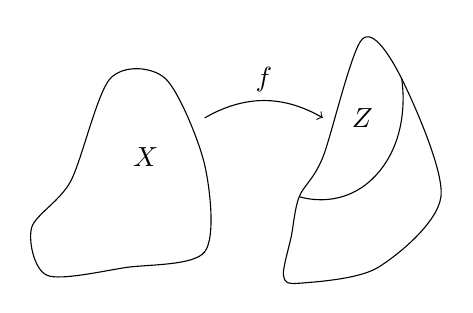
\begin{tikzpicture}
		\draw plot [smooth cycle] coordinates {(0,0) (1,0.1) 
		(2,0.3) (2,1.4) (1.5,2.5) (0.8,2.5) (0.3,1.2) (-0.2,0.6) } 
		node at (1.25,1.5) {$X$};
	
		\draw plot [smooth cycle] coordinates { (3,0) (3.1,.5) 
		(3.2,1) (3.5,1.5) (4,3) (4.5,2.5) (5,1) (4.2,.1) (3.2,-.1) 
		};
	
		\draw plot [smooth,tension=1.2] coordinates {(3.2,1) 
		(4.2,1.3) (4.5,2.5)} node at (4,2) {$Z$};
	
		\draw[->] (2,2) to [out=30,in=150] (3.5,2) node[above] at 
		(2.75,2.2) {$f$};
	\end{tikzpicture}
	\caption{If $f':X \to Z$ is a homeomorphism of $X$ with $Z$, 
	then $f'$ is a topological imbedding of $X$ in $Y$.}\label{top 
	imb}
\end{marginfigure}

\begin{definition}[Topological Imbedding]
	Suppose $f:X \to Y$ is an injective continuous map. Let $Z$ be 
	the image set $f(X)$, considered as a subspace of $Y$; then the 
	function $f':X \to Z$ obtained by restricting the range of $f$ 
	is bijective. If $f'$ happens to be a homeomorphism of $X$ with 
	$Z$, we say that the map $f:X \to Y$ is a \df{topological 
	imbedding}\index{topology!imbedding} of $X$ in $Y$.
\end{definition}

Figure \ref{top imb} illustrates this definition. Intuitively, the 
imbedding lets us treat $X$ as a subspace of $Y$ even though $X$ 
isn't a subset of $Y$.






























